%%%%%%%%%%%%%%%%%%%%%%%%%%%%%%%%%%%%%%%%%
% Beamer Presentation
% LaTeX Template
% Version 1.0 (10/11/12)
%
% This template has been downloaded from:
% http://www.LaTeXTemplates.com
%
% License:
% CC BY-NC-SA 3.0 (http://creativecommons.org/licenses/by-nc-sa/3.0/)
%
%%%%%%%%%%%%%%%%%%%%%%%%%%%%%%%%%%%%%%%%%

%----------------------------------------------------------------------------------------
%	PACKAGES AND THEMES
%----------------------------------------------------------------------------------------

\documentclass[usenames,dvipsnames,table]{beamer}

\mode<presentation> {

\usetheme{Madrid}
%\setbeamertemplate{footline} % To remove the footer line in all slides uncomment this line
%\setbeamertemplate{footline}[page number] % To replace the footer line in all slides with a simple slide count uncomment this line
\setbeamertemplate{navigation symbols}{} % To remove the navigation symbols from the bottom of all slides uncomment this line
}

\usepackage{amsmath}
\usepackage{graphicx} % Allows including images
\usepackage{booktabs} % Allows the use of \toprule, \midrule and \bottomrule in tables
\usepackage{listings}
\usepackage{xcolor}
\usepackage{xfrac}
% \usepackage{enumitem}

\usefonttheme[onlymath]{serif}

%----------------------------------------------------------------------------------------
%	TITLE PAGE
%----------------------------------------------------------------------------------------

\title[ABDA Ch 10]{Applied Bayesian Data Analysis --- Chapter 10}

\author{Kim Albertsson} % Your name
\institute[LTU and CERN]
{
CERN and Luleå University of Technology \\
\medskip
\textit{kim.albertsson@ltu.se}
}
\date{\today}

\newcommand{\cgy}{\cellcolor{gray!25}}
\newcommand{\cgr}{\cellcolor{green!25}}
\newcommand{\cye}{\cellcolor{orange!25}}
\newcommand{\ccb}{\cellcolor{Cerulean!25}}

\begin{document}

\begin{frame}
\titlepage % Print the title page as the first slide
\end{frame}

% \begin{frame}
% \frametitle{}
% \begin{itemize}
% \item
% \end{itemize}
% \end{frame}

%----------------------------------------------------------------------------------------
%	PRESENTATION SLIDES
%----------------------------------------------------------------------------------------
\section{Chapter 10}
\begin{frame}
\begin{center}
{\huge{Chapter 10}}
\\\vspace{2em}
Model comparison and Hierarchical Modelling
\vspace{5em}
\end{center}
\end{frame}


\begin{frame}
\frametitle{Introduction}

Occam's razor: Simple models are preferred.

\vspace{1em}
How to measure? Model comparison!

\vspace{1em}
(Can be) cast as a hierarchical modelling problem over a categorical variable.

\vspace{1em}
\textbf{Note:} Model, for model comparison, given by $\theta, p(\mathbf{y} | \theta)$
               and $p(\theta)$. Sensitive to choice of $p(\theta)$!

\vspace{2em}
\textbf{Note:} A categorical variable is a discrete variable lacking
               \emph{order}. I.e. the output can be shuffled without a change
               in semantics.

\end{frame}



\begin{frame}
\frametitle{General Formula and the Bayes Factor}
Introduce categorical varibale $m={1, 2, \ldots}$ for model.
\begin{align*}
\text{Posterior }           & p_m(\theta_1, \theta_2, \ldots, m|\mathbf{y}) \\
\text{Likelihood }          & p_m(\mathbf{y}| \theta_m, m) \\
\text{Prior }               & p_m(\theta_m| m) \\
\text{Model (hyper-)prior } & p(m)
\end{align*}

\textbf{Note:} Having both subscript and argument above is for mathematical
               convenience.
\begin{align*}
p_m(\cdot, M=m') =
    \begin{cases}
    p_m(\cdot) \text{ if } m = m' \\
    0, \text{ otherwise}
    \end{cases}
\end{align*}
\end{frame}




\begin{frame}
\frametitle{Model Comparison as a Single Hierarchical Model}
\begin{figure}
\centering
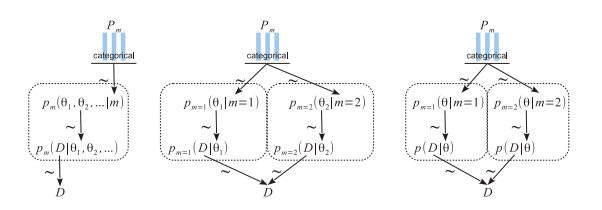
\includegraphics[width=\textwidth]{img/fig10_1}
\end{figure}
\begin{columns}[t]
\column{.3\textwidth}
\textbf{Left}
Joint model space.

\column{.3\textwidth}
\textbf{Middle}
Expanded example of joint space when number of models is two.

\column{.3\textwidth}
\textbf{Right}
Special case: Compare only priors.
\end{columns}
\end{frame}




\begin{frame}
\frametitle{Posterior (I)}

With
\begin{align*}
p_m(\cdot, M=m') =
    \begin{cases}
    p_m(\cdot) \text{ if } m = m' \\
    1, \text{ otherwise}
    \end{cases},
\end{align*}
and by definition
\begin{align*}
p(\theta_1, \theta_2, \ldots, 1|\mathbf{y})
    &\propto p_1(\mathbf{y}|\theta_1, 1)
             p(\theta_1, 1)
\\
p(\theta_1, \theta_2, \ldots, 2|\mathbf{y})
    &\propto p_2(\mathbf{y}|\theta_2, 2)
             p_2(\theta_2, 2)
.
\end{align*}
Thus the posterior is proportional to (loop over all models)
\begin{align*}
p(\theta_1, \theta_2, \ldots, m|\mathbf{y})
    &\propto p(\mathbf{y}|\theta_1, \theta_2, \ldots, m)
             p(\theta_1, \theta_2, \ldots, m)
\\
    &\propto p(\mathbf{y}|\theta_1, \theta_2, \ldots, m)
             p(\theta_1, \theta_2, \ldots| m)
             p(m)
\\
    &\propto p(m)
             \prod_{m^*} p_{m^*}(\mathbf{y}|\theta_{m^*}, m)
                         p_{m^*}(\theta_{m^*}| m).
\end{align*}

\end{frame}

\begin{frame}
\frametitle{Posterior (II)}

Finally
\begin{align*}
    & p(\theta_1, \theta_2, \ldots, m|\mathbf{y}) =
\\
    & \qquad\qquad
      \frac{p(m)
            \prod_{m^*} p_{m^*}(\mathbf{y}|\theta_{m^*}, m)
                        p_{m^*}(\theta_{m^*}| m)}
           {\sum_{m'} \int\! d\theta_{m'}
            p(m')
            \prod_{m^*} p_{m^*}(\mathbf{y}|\theta_{m^*}, m')
                        p_{m^*}(\theta_{m^*}| m')} \tag{10.2*}
\end{align*}

\vspace{3em}
\begin{color}{gray}
Contrast to eqn. in book (handwavy!)
\begin{align*}
    & p(\theta_1, \theta_2, \ldots, m|\mathbf{y}) =
\\
    & \qquad\qquad
      \frac{\prod_{m} p_m(\mathbf{y}|\theta_m, m)
                        p_{m}(\theta_m| m)p(m)}
           {\sum_m \int\! d\theta_m\
            \prod_m p_m(\mathbf{y}|\theta_m, m)
                        p_m(\theta_m| m)p(m)} \tag{10.2}
\end{align*}
\end{color}

\end{frame}

\begin{frame}
\frametitle{Alternative Posterior}

Alternative formulation
\begin{align*}
p(\theta_1, \theta_2, \ldots, m|\mathbf{y})
    &\propto p(\mathbf{y}|\theta_1, \theta_2, \ldots, m)
             p(\theta_1, \theta_2, \ldots, m)
\\
    &\propto p(\mathbf{y}|\theta_1, \theta_2, \ldots, m)
             p(\theta_1, \theta_2, \ldots| m)
             p(m)
\\
    &\propto \sum_{m^*} 1_{m^*}(m) p_{m^*}(\mathbf{y}|\theta_{m^*})
                                   p_{m^*}(\theta_{m^*})p(m)
\\
    &\propto p_{m}(\mathbf{y}|\theta_{m}) p_{m}(\theta_{m})p(m).
\end{align*}

Thus
\begin{align*}
p(\theta_1, \theta_2, \ldots, m|\mathbf{y})
    &= \frac{p_{m}(\mathbf{y}|\theta_{m}) p_{m}(\theta_{m})p(m)}
            {\sum_{m'} \int\! d\theta_{m'}\
             p_{m'}(\mathbf{y}|\theta_{m'}) p_{m'}(\theta_{m'})p(m')}\tag{10.2*}.
\end{align*}
For me, this is clearer.
\end{frame}



\begin{frame}
\frametitle{Model posterior}

Model posterior:
\begin{align*}
p(m|\mathbf{y})
    &= \frac{p(\mathbf{y}|m)p(m)}
            {\sum_{m'} p(\mathbf{y}|m')p(m')}, \tag{10.3}
\end{align*}

where
\begin{align*}
p(\mathbf{y}|m)
    &= \int\! d\theta_{m}\,
             p_{m}(\mathbf{y}|\theta_{m},m) p_{m}(\theta_{m}|m). \tag{10.4}
\end{align*}

\textbf{Key point:} A model is a tuple: \texttt{(likelihood, prior)}! (We marginalise across both likelihood and prior to arrive at the model posterior.)
\end{frame}

\begin{frame}
\frametitle{Bayes Factor}

Consider the relative posterior probabilities (posterior odds):
\begin{align*}
\frac{p(m_0|\mathbf{y})}
     {p(m_1|\mathbf{y})}
    &=  \underbrace{\frac{p(\mathbf{y}|m_0)}
                         {p(\mathbf{y}|m_1)}}_{\textrm{BF}}
        \frac{p(m_0)}
             {p(m_1)}
        \underbrace{\frac{/\sum_{m'}p(\mathbf{y}|m')p(m')}
                         {/\sum_{m'}p(\mathbf{y}|m')p(m')}}_{=1}
\tag{10.5}
\end{align*}
The Bayes Factor ($\mathrm{BF}$) is ratio of the probabilities of the data (under the two models).
\begin{align*}
\textrm{posterior odds} = \textrm{BF} \cdot \textrm{prior odds}
\end{align*}
\emph{\textrm{``How much the prior odds change given the data''}}

\end{frame}



\begin{frame}
\frametitle{Example of two factories of coins}
\begin{columns}[c]
\column{.5\textwidth}
For the following we'll use model of two factories having different expected means of the coin bias.

\vspace{1em}
Goal: Find out what factory produced the coin.
\column{.5\textwidth}
\begin{figure}
\centering
\vspace{-1em}
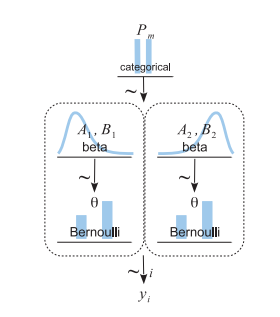
\includegraphics[width=\textwidth]{img/fig10_2}
\end{figure}
\end{columns}
\end{frame}






\begin{frame}
\frametitle{10.2.2 Solution by grid approximation}
\begin{columns}[c]
\column{.5\textwidth}
Discretisize joint model (possible b.c. small)

\vspace{1em}
Yields Bayes factor estimate similar to analytical method: $\sim 5:1$.
\column{.5\textwidth}
\begin{figure}
\centering
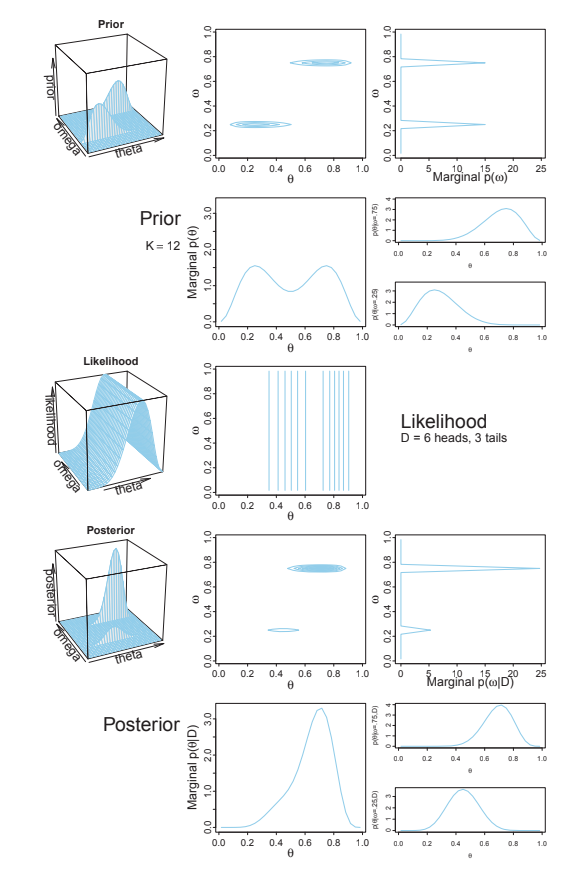
\includegraphics[height=.8\textheight]{img/fig10_3}
\end{figure}
\end{columns}
\end{frame}




\begin{frame}
\frametitle{10.2.1 Solution by formal analysis}

We can calculate the Bayes factor with
\begin{align*}
p(\mathbf{y}|m) = p(z, N) = \frac{B(z+a_m, N-z+b_m)}{B(a_m, b_m)} \tag{10.6}
\end{align*}
(But use logarithm rewrite for numerical stability!)

\begin{align*}
\frac{p(m_0|\mathbf{y})}
     {p(m_1|\mathbf{y})}
    =  \frac{p(\mathbf{y}|m_0)}
             {p(\mathbf{y}|m_1)}
        \frac{p(m_0)}
             {p(m_1)}
    =  \frac{0.000499}
             {0.002339}
        \frac{0.5}
             {0.5}
    = 0.213
\end{align*}
\textbf{Note:} In this analysis, posterior only over $m$! Use previously developed techniques for estimating $\theta$!

\end{frame}




\begin{frame}
\frametitle{10.3 Solution by MCMC}
Idea 1: Estimate $p(\mathbf{y}|m)$ for each model independently and calculate Bayes factor. Use variation of
\begin{align*}
p(\mathbf{y}) &= \int\! d\theta\, p(\mathbf{y}|\theta) p(\theta) \\
              &\approx \frac{1}{N}\sum_{\theta_i \sim p(\theta)}^N p(\mathbf{y}|\theta_i).
\end{align*}
Problematic for complex models.

\vspace{1em}
Idea 2: Cast problem as a hierarchical one, including $m$. Calculate bayes factor by simple statistic. Can have convergence problems due to autocorrelation.
\end{frame}




\begin{frame}
\frametitle{10.3.1 Non-hierarchical MCM computation of each mdoel's marginal likelihood}

Idea 1: Estimate $p(\mathbf{y}|m)$ for each model independently and calculate Bayes factor.
\begin{align*}
p(\mathbf{y}) &= \int\! d\theta\, p(\mathbf{y}|\theta) p(\theta)
              \approx \frac{1}{N}\sum_{\theta_i \sim p(\theta)}^N p(\mathbf{y}|\theta_i).
\end{align*}
However, usually $p(\mathbf{y}|\theta)$ is nearly zero for many values of $\theta$. Use trick
\begin{align*}
\frac{1}{p(\mathbf{y})} &= \frac{p(\theta|\mathbf{y})}
                                {p(\mathbf{y}|\theta) p(\theta)} \\
                        &= \int\! d\theta\, \frac{h(\theta)}
                                                 {p(\mathbf{y}|\theta) p(\theta)}
                                            p(\theta|\mathbf{y})
              \approx \frac{1}{N}\sum_{\theta_i \sim p(\theta)}^N
                       \frac{h(\theta)}
                            {p(\mathbf{y}|\theta_i) p(\theta_i)}.
\end{align*}
\textbf{Note:} For numerical statbility, choose $h(\theta_i)$ close to posterior, but can be tricky for high-dimensional models.
\end{frame}


\begin{frame}
\frametitle{10.3.2 Hierarchical MCMC computation of relative model probability}
\begin{columns}[c]
\column{.5\textwidth}

\begin{align*}
\frac{p(m_0|\mathbf{y})}
     {p(m_1|\mathbf{y})}
    =  \frac{0.177}
             {0.823}
    = 0.215
\end{align*}

However, problems with autocorrelation and skewed visitation of $m$.

\column{.5\textwidth}
\begin{figure}
\centering
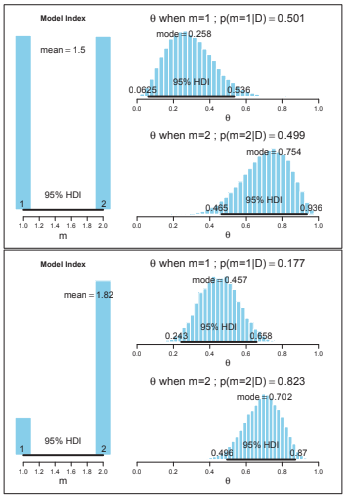
\includegraphics[height=.8\textheight]{img/fig10_4}
\end{figure}
\end{columns}
\end{frame}


\begin{frame}
\frametitle{Poor jumping when not using pseudo-priors}
\begin{columns}[c]
\column{.5\textwidth}

When $M=1$, $\theta_1$ is sampled from it's posterior, but $\theta_2$ is sampled from its prior.

\vspace{1em}
When sampling $m$ (lockstep) a jump is likely to be rejected since $\theta_2$ does not describe the data well.

\column{.5\textwidth}
\begin{figure}
\centering
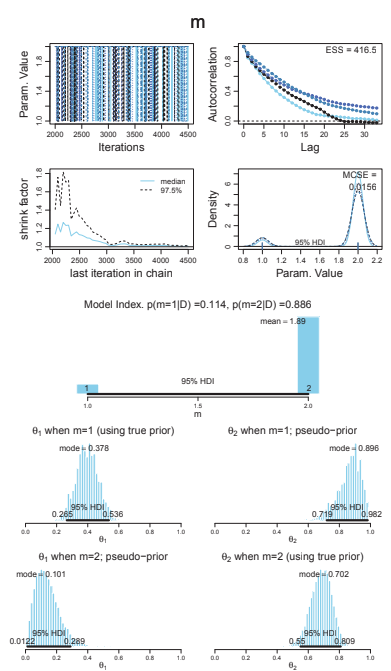
\includegraphics[height=.8\textheight]{img/fig10_5}
\end{figure}
\end{columns}
\end{frame}


\begin{frame}
\frametitle{Better jumping with pseudo-priors}
\begin{columns}[c]
\column{.5\textwidth}
Introduce pseudo-priors, which change the sampling distribution when $m$ does not correspond to the model.

\vspace{1em}
If chosen close to posterior, jump is likely. Choose by iterative process.

\begin{align*}
\frac{p(m_0|\mathbf{y})}
     {p(m_1|\mathbf{y})}
    =  \frac{0.114}
             {0.886}
    = 0.129 \text{ (!?)}
\end{align*}

\vspace{1em}
Q: Why does this not change the final distribution?
\column{.5\textwidth}
\begin{figure}
\centering
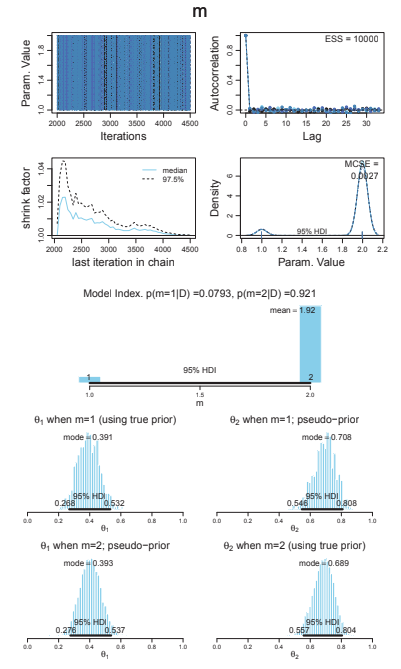
\includegraphics[height=.8\textheight]{img/fig10_6}
\end{figure}
\end{columns}
\end{frame}





\begin{frame}
\frametitle{10.4 Prediciton: Model Averaging}

The full posterior is the best description available.
\begin{align*}
p(\hat{y}|D, M=b)
    &= \int\! d\theta_b\, p_b(\hat{y}|\theta_b, M=b)p_b(\theta_b|\mathbf{y}, M=b)\\
\end{align*}%
\begin{center}vs.\end{center}%
\begin{align*}
p(\hat{y}|D)
    &= \sum_m \int\! d\theta_m\, p_m(\hat{y}|\theta_m, M=m)p_m(\theta_m|\mathbf{y}, M=m) p(M=m)\\
\end{align*}
\end{frame}





\begin{frame}
\frametitle{10.5 Model complexity naturally accounted for}
Bayesian modeling naturally accounts for model complexity.

\vspace{1em}
Complex models, with large paramter space, $\implies$ probability density spread out across probabilties.

\vspace{1em}
Key: Prior important!
\begin{align*}
\frac{p(m_0|\mathbf{y})}
     {p(m_1|\mathbf{y})}
    =  \frac{p(\mathbf{y}|m_0)}
             {p(\mathbf{y}|m_1)}
        \frac{p(m_0)}
             {p(m_1)}
\end{align*}

\begin{align*}
p(\mathbf{y}|m)
    &= \int\! d\theta_{m}\,
             p_{m}(\mathbf{y}|\theta_{m},m) p_{m}(\theta_{m}|m). \tag{10.4}
\end{align*}

\begin{align*}
\end{align*}
\end{frame}






% \begin{frame}
% \frametitle{10.5.1 Caveats regarding nested model comparison}

% \begin{align*}
% \end{align*}
% \end{frame}







\begin{frame}
\frametitle{10.6 Extreme sensitivity to prior distribution}

Vague priors with vastly different density distributions.
\begin{align*}
\mathrm{beta}(1, 1)\\
\mathrm{beta}(.1, .1)
\end{align*}

Marginalise across likelihood and prior.
\begin{align*}
p(\mathbf{y}|m)
    &= \int\! d\theta_{m}\,
             p_{m}(\mathbf{y}|\theta_{m},m) p_{m}(\theta_{m}|m). \tag{10.4}
\end{align*}

\end{frame}





\begin{frame}
\frametitle{10.6.1 Priors of different models should be equally informed}
Prior should model our beliefs about distribution under data.

\vspace{1em}
Use parts of the dataset to inform priors. This overwhelms any "vague" prior.

\vspace{1em}
Calculate the posterior for each model individually ($\sim 10\%$ of data) and use that as prior for model comparison.

\begin{align*}
\end{align*}
\end{frame}




\end{document} 